\section{Connectedness}
\label{sect:connectedness}
\subsection{Connectedness}
\label{subsect:connectedness}
\begin{enumerate}
\item We have generalized the \emph{extreme value theorem} in
\Cref{thm:cts-cpt-evt}. Then the next natural thing to do is to generalize the
\emph{intermediate value theorem} we learn in MATH2241. It turns out that the
generalization uses the notion of \emph{connectedness}.

\item It is somehow complicated to directly define the concept of
connectedness. So, we shall first define the notion of
\underline{dis}connectedness, and then define connectedness as the state of
being \emph{not} disconnected.

\item A metric space \(X\) is said to be \defn{disconnected} if \(X=A\sqcup B\)
for some nonempty and disjoint sets \(A\) and \(B\) which are open in \(X\).  A
metric space \(X\) is said to be \defn{connected} if it is not disconnected. A
subset \(S\) of \(X\) is said to be \defn{connected} (in \(X\)) if it is
connected when considered as a metric space itself under the induced metric.

Example: \(X=[0,1]\cup [2,3]\) (equipped with standard Euclidean metric) is
disconnected, by noting that \([0,1]\) and \([2,3]\) are nonempty disjoint open
subsets of \(X\) whose union is \(X\).

\item The following gives several criteria for being disconnected.

\begin{proposition}
\label{prp:discon-crit}
Let \(X\) be a metric space. The following are equivalent.
\begin{enumerate}
\item \(X\) is disconnected, i.e., \(X=A\sqcup B\) for some nonempty and
disjoint sets \(A\) and \(B\) which are \emph{open} in \(X\).
\item \(X=A\sqcup B\) for some nonempty and
disjoint sets \(A\) and \(B\) which are \emph{closed} in \(X\).
\item There exists a proper nonempty closed and open subset of \(X\).
\end{enumerate}
\end{proposition}
\begin{pf}
\underline{\(\text{(a)}\implies \text{(b)}\)}: Assume that \(X=A\sqcup B\) for some nonempty and
disjoint sets \(A\) and \(B\) which are \emph{open} in \(X\). Note that as
complements of each other, \(B=X\setminus A\) and \(A=X\setminus B\) are also
\emph{closed} in \(X\).

\underline{\(\text{(b)}\implies \text{(c)}\)}: Assume that \(X=A\sqcup B\) for
some nonempty and disjoint sets \(A\) and \(B\) which are \emph{closed} in
\(X\). Then \(A=X\setminus B\) is open in \(X\). Since \(B\) is nonempty,
\(A=X\setminus B\) is a \emph{proper} subset of \(X\). It then follows that
\(A\) is a proper nonempty closed and open subset of \(X\).

\underline{\(\text{(c)}\implies \text{(a)}\)}: Assume that there exists a
proper nonempty closed and open subset of \(X\). Define \(B=X\setminus A\).
Since \(A\) is a \emph{proper} subset of \(X\), the set \(B\) is nonempty.
Furthermore, since \(A\) is closed in \(X\), \(B=X\setminus A\) is open in
\(X\). Also, we can see that \(A\cap B=\varnothing\) and \(X=A\sqcup B\).
\end{pf}

\item To prove that a metric space is \underline{dis}connected, we can just
find an example of \(A\) and \(B\) satisfying the specified conditions. On the
other hand, it is much more difficult to prove that a metric space is
connected, since we need to show that there \emph{do not exist} any such sets
\(A\) and \(B\). We need to consider all possible choices!

To simplify the arguments, the use of a continuous function which takes only
two possible values is very helpful.

\item Any continuous function from \(X\) to \(\{0,1\}\) equipped with discrete
metric is called a \defn{2-valued function} on \(X\). The following result
suggests how 2-valued function can help us to prove connectedness.

\begin{theorem}
\label{thm:conn-2-val}
A metric space \(X\) is connected iff the only possible 2-valued functions on
\(X\) are constant functions.
\end{theorem}
\begin{pf}
``\(\Leftarrow\)'': We prove by contrapositive. Assume that \(X\) is
disconnected. Then we can write \(X=A\sqcup B\) for some nonempty and disjoint
sets \(A\) and \(B\) which are open in \(X\). Then define a function
\(f:X\to\{0,1\}\), where \(\{0,1\}\) is equipped with discrete metric, by
\[
f(x)=\begin{cases}
0&\text{if \(x\in A\)},\\
1&\text{if \(x\in B\)}.
\end{cases}
\]
Note that every subset of \(\{0,1\}\) is open.  Then we can check that
\(f^{-1}(\varnothing)=\varnothing\), \(f^{-1}(\{0\})=A\), \(f^{-1}(\{1\})=B\), and
\(f^{-1}(\{0,1\})=A\sqcup B=X\) are all open in \(X\). Thus, \(f\) is
continuous, hence is a non-constant 2-valued function.


``\(\Rightarrow\)'': Assume that \(X\) is connected.  Let \(f:X\to\{0,1\}\) be
a 2-valued function. Assume to the contrary that \(f\) is non-constant. Then
the preimages \(f^{-1}(\{0\})\) and \(f^{-1}(\{1\})\) are both nonempty. Also,
due to the continuity of \(f\), the preimages are both open in \(X\). Note also
that \(f^{-1}(\{0\})\cap f^{-1}(\{1\})=\varnothing\). Thus, we can write
\[
X=f^{-1}(\{0\})\sqcup f^{-1}(\{1\}),
\]
which implies that \(X\) is disconnected, contradiction.
\end{pf}

\item Like compactness, \emph{connectedness} is also preserved by continuous
functions by the following result.

\begin{proposition}
\label{prp:cts-preserv-conn}
Let \(f:X\to Y\) be a continuous function and \(S\subseteq X\) be a connected
set in \(X\). Then, the image \(f(S)\) is connected in \(Y\).
\end{proposition}
\begin{pf}
Let \(g:f(S)\to\{0,1\}\) be any 2-valued function on \(f(S)\). Then, due to the
continuity of both \(f\) and \(g\), the composition \(g\circ f:X\to \{0,1\}\)
is also continuous, so is the restriction \(g\circ f|_{S}:S\to\{0,1\}\). But
then it just means that \(g\circ f|_{S}:S\to\{0,1\}\) is a 2-valued function on
\(S\).

Due to the connectedness of \(S\), \(g\circ f|_{S}\) must be a constant
function. It then forces \(g\) to be a constant function as well, hence
\(f(S)\) is connected.
\end{pf}

Particularly, this implies that connectedness is a topological property, i.e.,
preserved by homeomorphisms.

\item We can then generalize the intermediate value theorem we learn in MATH2241.
\begin{theorem}[Intermediate value theorem]
\label{thm:ivt-conn}
Let \(f:X\to\R\) be a continuous function on a connected metric space \(X\). If
\(f\) takes on two different values \(a,b\in X\), then \(f\) takes on every
real number \(c\in[a,b]\), i.e., for any \(c\in[a,b]\), there exists \(x\in X\)
such that \(f(x)=c\).
\end{theorem}
\begin{pf}
Since \(f\) is continuous and \(X\) is connected, by
\Cref{prp:cts-preserv-conn} we know that \(f(X)\) is connected in \(\R\).
Now assume to the contrary that there exist \(c\in [a,b]\) such that
\(f(x)\ne c\) for any \(x\in X\). Indeed, we have \(c\in (a,b)\) since \(f\)
takes on \(a\) and \(b\) by assumption.

Then, define \(A=(-\infty,c)\cap f(X)\) and \(B=(c,\infty)\cap f(X)\).
\begin{center}
\begin{tikzpicture}
\draw[-Latex] (0,0) -- (10,0);
\node[] () at (3,-0.5) {\(a\)};
\node[] () at (7,-0.5) {\(b\)};
\node[red] () at (5,-0.5) {\(c\)};
\draw[red] (5,0) circle [radius=0.7mm];
\node[blue] () at (2,0) {(};
\node[blue] () at (4.95,0) {)};
\node[green!50!black] () at (5.05,0) {(};
\node[green!50!black] () at (9,0) {)};
\node[blue] () at (3.5,0.4) {\(A\)};
\node[green!50!black] () at (7,0.4) {\(B\)};
\draw[orange, opacity=0.3, line width=1mm, line cap=round] (2,0) -- (4.88,0);
\draw[orange, opacity=0.3, line width=1mm, line cap=round] (5.12,0) -- (9,0);
\node[orange, opacity=0.7] () at (5,0.5) {\(f(X)\)};
\end{tikzpicture}
\end{center}
Note that we have \(f(X)=A\sqcup B\) where \(A\) and \(B\) are nonempty
disjoint open subsets of \(f(X)\), thus \(f(X)\) is disconnected,
contradiction.
\end{pf}

\item The next result concerns the connectedness of union of connected sets. It
turns out that, similar to openness, arbitrary union of connected sets is
connected, \emph{provided that} the connected sets involved have nonempty
intersection.
\begin{proposition}
\label{prp:conn-union-nonemp-int-conn}
Let \(\{U_{\alpha}\}_{\alpha\in\Lambda}\) be a collection of connected
subsets of \(X\) with \(\bigcap_{\alpha\in\Lambda}U_{\alpha}\ne\varnothing\).
Then, the union \(\bigcup_{\alpha\in\Lambda}U_{\alpha}\) is connected.
\end{proposition}
\begin{pf}
Fix any \(t\in\bigcap_{\alpha\in\Lambda}U_{\alpha}\) and let
\(f:\bigcup_{\alpha\in\Lambda}\to\{0,1\}\) be a 2-valued function on
\(\bigcup_{\alpha\in\Lambda}\). Then for any \(\beta\in\Lambda\), the
restriction \(f|_{U_{\beta}}:U_{\beta}\to\{0,1\}\) is a 2-valued function on
\(U_{\beta}\). Since \(U_{\beta}\) is connected, \(f|_{U_{\beta}}\) must be a
constant function by \Cref{thm:conn-2-val}. Particularly, we must have
\(f(x)=f(t)\) for any \(x\in U_{\beta}\), since \(t\) is always an element of
\(U_{\beta}\).

Since this holds for any \(\beta\in\Lambda\), we conclude that \(f(x)=f(t)\)
for any \(x\in\bigcup_{\alpha\in\Lambda}U_{\alpha}\), thus \(f\) is a constant
function. So, by \Cref{thm:conn-2-val}, \(\bigcup_{\alpha\in\Lambda}U_{\alpha}\)
is connected.
\end{pf}

\item Recall from \Cref{thm:union-disjoint-int} that every nonempty open subset
of \(\R\) can be expressed as the union of countably many disjoint open
intervals in \(\R\) uniquely. Using the notion of connectedness, we can obtain
a corresponding result in \(\R^n\). In the case for proving
\Cref{thm:union-disjoint-int}, we have utilized the notion of \emph{maximal
open interval}. Here, we need an analogous notion. A maximal connected set in a
metric space is called a \defn{connected component} of the metric space.

Here, maximality of a connected set \(S\) in a metric space \(X\) means that
for any connected set \(T\) in \(X\) with \(T\supseteq S\), we have \(T=S\).
There is not a connected set in \(X\) that is a \emph{proper superset} of
\(S\). In particular, this implies a connected component must be nonempty,
since any singleton is a connected set in \(X\), which is a proper superset of
an empty set.

\item Like the case for \(\R\), such maximal connected set is indeed a certain
union. To be more precise, we have the following result.

\begin{proposition}
\label{prp:conn-comp-union}
Let \(X\) be a metric space, \(x\in X\), and \(U_x\) be the union of
\underline{all} connected sets in \(X\) that contain \(x\). Then, \(U_x\) is
the unique connected component of \(X\) that contains \(x\).
\end{proposition}
\begin{pf}
First we show that \(U_x\) is a connected component of \(X\). Note that \(U_x\)
is nonempty since at least \(\{x\}\) is a connected set containing \(x\). Thus,
by \Cref{prp:conn-union-nonemp-int-conn}, \(U_x\) is connected. Since every
connected set in \(X\) that contains \(x\) must be a subset of the union
\(U_x\), the union \(U_x\) is indeed a maximal connected set in \(X\), thus a
connected component of \(X\).

Next we prove the uniqueness. Suppose that \(V_x\) is also a connected
component of \(X\) that contains \(x\). Then in particular, \(V_x\) is a
connected set in \(X\) that contains \(x\), thus \(V_x\subseteq U_x\). But then
by the maximality of \(V_x\), we must have \(U_x=V_x\), establishing the
uniqueness.
\end{pf}

Consider any connected component \(U\) of \(X\) and pick any \(x\in U\). By
\Cref{prp:conn-comp-union}, we know that the union of all connected sets in
\(X\) that contain \(x\), i.e., \(U_x\), is the unique connected component of
\(X\) that contains \(x\). This then means that \(U\) is just given by this
unique connected component \(U_x\).

\item \label{it:conn-compo-ident-or-disjoint}
Observe that connected components of \(X\) are either identical or disjoint.

\begin{pf}
The proof is similar to the one for the corresponding property in
\Cref{lma:open-int-union-int}. Here again we will prove that given any two
connected components \(U_x\) and \(U_y\), if \(U_x\cap U_y\ne\varnothing\),
then \(U_x=U_y\). Here the notations \(U_x\) and \(U_y\) carry the meaning
suggested in \Cref{prp:conn-comp-union}.

Firstly, since \(U_x\) and \(U_y\) are connected with nonempty intersection,
\(U_x\cup U_y\) is connected also, and contains \(x\).  By the maximality of
\(U_x\) and \(U_y\) respectively, we have \(U_x\cup U_y\subseteq U_x\) and
\(U_x\cup U_y\subseteq U_y\). This implies that \(U_x\cup U_y=U_x\) and
\(U_x\cup U_y=U_y\) as another subset inclusion always holds. Thus,
\(U_x=U_y\).
\end{pf}

\item \label{it:expr-disjoint-union-conn-compo} By going through all elements
in any subset \(S\) of \(X\) and applying \Cref{prp:conn-comp-union} for each
of them, we can obtain a unique collection of disjoint connected components of
\(S\) whose union is \(S\), which contains all distinct connected components of
\(S\). In other words, \(S\) can always be uniquely decomposed into a disjoint
union of connected components of \(S\).

\item Next we will introduce some properties of connected components. Before
that, we consider the following lemmas.
\begin{lemma}
\label{lma:set-btw-s-clos-conn}
If \(S\subseteq X\) is connected, then every \(T\subseteq X\) with \(S\subseteq
T\subseteq \overline{S}\) is connected.
\end{lemma}
\begin{pf}
Let \(f:T\to\{0,1\}\) be any 2-valued function on \(T\). Then the restriction
of \(f\) on \(S\subseteq T\), \(f|_S\), is a 2-valued function on \(S\). Since
\(S\) is connected, \(f|_S\) is constant by \Cref{thm:conn-2-val}. WLOG,
suppose that \(f|_S\equiv 0\). For any \(x\in T\subseteq \overline{S}\), there
exists a sequence \(\{x_n\}\) in \(S\) such that \(\{x_n\}\to x\), by
\Cref{prp:adher-accum-seq-equiv}. Then by the continuity of \(f\), we have
\(f(x)=\lim_{n\to \infty}f(x_n)=\lim_{n\to \infty}0=0\), by
\Cref{prp:cts-seq-lim-crit}.
\end{pf}
\begin{lemma}
\label{lma:int-conn}
A set \(I\subseteq \R\) is an interval iff it is connected.
\end{lemma}
\begin{pf}
``\(\Leftarrow\)'': We prove by contrapositive. Assume that \(I\) is not an
interval. Then, there exists \(c\in (a,b)\) with \(a,b\in I\) and \(c\notin
I\). Define \(A=(-\infty,c)\cap I\) and \(B=(c,\infty)\cap I\), which are
nonempty disjoint open subsets of \(I\). By writing \(I=A\sqcup B\),
we know that \(I\) is disconnected.

``\(\Rightarrow\)'': Let \(I\subseteq \R\) be an interval. If \(I\) is a
singleton, there is nothing to prove. So henceforth assume that \(I\) is a
nondegenerate interval, i.e., one that has more than one element.

Let \(f:I\to\{0,1\}\) be any 2-valued function on \(I\). Assume to the contrary
that there are distinct points \(a,b\in I\) such that \(f(a)\ne f(b)\).  WLOG,
assume \(a<b\), \(f(a)=0\) and \(f(b)=1\). Since \(I\) is an interval, it
contains every value between \(a\) and \(b\) also, i.e., \([a,b]\subseteq I\).

Let \(t=\inf\{x\in [a,b]:f(x)=1\}\). Then, \(t\in (a,b]\subseteq I\) and
\(f(x)=0\) for any \(x<t\) in \(I\). By the continuity of \(f\), we have
\(f(t)=\lim_{x\to t^{-}}f(x)=0\).

On the other hand, since infimum is a lower bound, for any \(n\in\N\), there
exists \(x_n\in [t+t+\frac{1}{n})\cap I\) such that \(f(x_n)=1\). Observe that
\(\{x_n\}\) is a sequence in \(I\) converging to \(t\), by sandwich theorem.
Thus, by \Cref{prp:cts-seq-lim-crit}, we have \(f(t)=\lim_{n\to
\infty}f(x_n)=1\), contradiction.
\end{pf}

\item With the help of \Cref{lma:set-btw-s-clos-conn,lma:int-conn}, we can
prove the following result about some properties of connected components.
\begin{proposition}
\label{prp:conn-compo-prop}
Let \(X\) be a metric space.
\begin{enumerate}
\item Every connected component of \(X\) is closed in \(X\).
\item Connected components of \(X\) may not be open in \(X\).
\item Every connected component of an open subset \(S\subseteq \R^n\) (as a
metric subspace) is open in \(\R^n\).
\end{enumerate}
\end{proposition}
\begin{pf}
\begin{enumerate}
\item Let \(S\) be any connected component of \(X\). By
\Cref{lma:set-btw-s-clos-conn}, \(\overline{S}\supseteq S\) is also connected.
By the maximality of \(S\), we then have \(\overline{S}=S\), meaning that \(S\)
is closed in \(X\) by \Cref{prp:equiv-crit-closed}.

\item Let \(X=\{\frac{1}{n}:n\in\N\}\cup\{0\}\). Since the only connected set
containing \(0\) is \(\{0\}\), the singleton \(\{0\}\) is a connected component
of \(X\). But it is not open in \(X\).

\item Let \(T\subseteq S\) be any connected component of \(S\). Then for any
\(x\in T\subseteq S\), due to the openness of \(S\), there exists \(r>0\) such
that the open ball \(B_{\R^n}(x,r)=B(x,r)\subseteq S\subseteq \R^n\).
\begin{center}
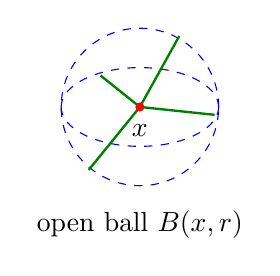
\begin{tikzpicture}
\draw[blue, dashed] (3,0) circle [radius=1cm];
\draw[blue, dashed] (2,0) arc (180:360:1 and 0.5);
\draw[blue, dashed] (4,0) arc (0:180:1 and 0.5);
\node[] () at (3,-0.3) {\(x\)};
\draw[green!50!black, line width=0.3mm] (3,0) -- (3.5,0.9);
\draw[green!50!black, line width=0.3mm] (3,0) -- (2.5,0.4);
\draw[green!50!black, line width=0.3mm] (3,0) -- (2.35,-0.8);
\draw[green!50!black, line width=0.3mm] (3,0) -- (3.95,-0.1);
\draw[red, fill] (3,0) circle [radius=0.5mm];
\node[] () at (3,-1.5) {open ball \(B(x,r)\)};
\end{tikzpicture}
\end{center}
Note that every radius of the open ball \(B(x,r)\) (\gc{green} line segments in
the picture above) is homeomorphic to the interval \([0,r)\subseteq \R\), which
is connected by \Cref{lma:int-conn}. Since connectedness is a topological
property, every radius is connected. Furthermore, the intersection of all the
radii is \(\{x\}\), thus nonempty. Noting that the open ball \(B(x,r)\) is
indeed the union of all the radii (with nonempty intersection), we conclude by
\Cref{prp:conn-union-nonemp-int-conn} that the open ball \(B(x,r)\) is
connected.

Since \(T\) contains \(x\), it must be the union of all connected sets
containing \(x\) by \Cref{prp:conn-comp-union}.  Hence, we must have
\(B(x,r)\subseteq T\). Thus, \(T\) is open in \(\R^n\).
\end{enumerate}
\end{pf}
\item To close \Cref{subsect:connectedness}, we will prove a result analogous
to \Cref{thm:union-disjoint-int} but for \(\R^n\) below.

\begin{theorem}
\label{thm:open-count-union-conn-compo}
Every nonempty open subset \(S\) of \(\R^{n}\) can be uniquely expressed as a
\emph{countable} disjoint union of nonempty open connected sets in \(\R^n\).
Furthermore, these open connected sets are all the connected components of
\(S\).
\end{theorem}
\begin{pf}
From \labelcref{it:expr-disjoint-union-conn-compo}, we know that \(S\) can be
expressed as a disjoint union of the connected components of \(S\). So to prove
the existence of such expression, it suffices to prove that (i) each connected
component is open in \(\R^n\), and (ii) the disjoint union is countable. Since
\(S\subseteq \R^n\), (i) follows from \Cref{prp:conn-compo-prop}.

Next, due to Lindel\"{o}f's theorem (\Cref{thm:lindelof}), we can assume
WLOG that such collection of connected components is countable, proving (ii).

It then remains to prove the uniqueness. Suppose we can write
\(S=\sqcup_{n=1}^{\infty}C_n\) where each \(C_n\) is a nonempty open connected
subset of \(S\). Consider any \(C_n\) and pick any \(x\in C_n\). Due to the
connectedness of \(C_n\), we know that \(C_n\subseteq U_x\) where \(U_x\)
denotes the connected component containing \(x\), i.e., the union of all
connected sets containing \(x\). Note that we can write \(C_n=S\setminus
\sqcup_{m\ne n}C_m\) where \(\sqcup_{m\ne n}C_m\) is open in \(S\) (as a union
of open sets), thus \(C_n\) is closed in \(S\) as well.

Since \(C_n\subseteq U_x\), this then implies that \(C_n=C_n\cap U_x\) is both
closed and open in \(U_x\), by
\labelcref{it:open-closed-equiv-crit-metric-subspace}. We claim that
\(C_n=U_x\). If this was not the case, i.e., \(C_n\) is a proper subset of
\(U_x\), then \(C_n\) would be a proper nonempty closed and open subset of
\(U_x\), which implies that \(U_x\) is disconnected by \Cref{prp:discon-crit},
contradiction. From this, we can deduce that the collection \(\{C_n\}\) is
indeed just the collection of all the connected components of \(S\). This proves the
uniqueness.
\end{pf}
\end{enumerate}
\subsection{Path-connectedness}
\label{subsect:path-conn}
\begin{enumerate}
\item In \Cref{subsect:path-conn}, we will discuss another notion of
``connectedness'', which is called path-connectedness. Recall that we have
defined connectedness as a state of being not disconnected. This is somewhat
indirect and may be unintuitive. In contrast, the concept of path-connectedness
is more direct and carries a clear geometric intuition. It turns out that
path-connectedness implies connectedness, so the former provides us an
``intuitive'' way to prove connectedness.

\item Before defining path-connectedness, we first define what a path is. A
\defn{path} in a metric space \(X\) is a continuous function \(\gamma:[0,1]\to
X\). For convenience, sometimes we call the image of \(\gamma\)
(\(\gamma([0,1])\)) as path also.

In the latter sense of path, every path in \(X\) would be a connected set in
\(X\). This is because \([0,1]\) is connected (as an interval; see
\Cref{lma:int-conn}) and continuous function preserves connectedness
(\Cref{prp:cts-preserv-conn}).

\item Two paths can be ``joined'' to form another path. If \(\alpha:[0,1]\to
X\) and \(\beta:[0,1]\to X\) are paths with \(\alpha(0)=p\),
\(\alpha(1)=\beta(0)=q\) (``ending point'' of \(\alpha\) = ``starting point''
of \(\beta\)), and \(\beta(1)=r\), then the function \(\gamma:[0,1]\to X\)
defined by
\[
\gamma(t)=\begin{cases}
\alpha(2t)&\text{if \(0\le t\le 1/2\)},\\
\beta(2t-1)&\text{if \(1/2\le t\le 1\)}
\end{cases}
\]
is a path in \(X\) joining \(p\) to \(r\) through \(\alpha\) and \(\beta\).
\begin{center}
\begin{tikzpicture}
\draw[blue, fill] (0,0) circle [radius=0.5mm];
\draw[blue, fill] (2,1) circle [radius=0.5mm];
\draw[blue, fill] (4,-0.5) circle [radius=0.5mm];
\draw[violet] (0,0) .. controls (0.4,-0.5) and (1.2,0) .. (2,1);
\node[violet] () at (1,-0.7) {\(\alpha\)};
\draw[brown] (2,1) .. controls (3,0.7) and (3.6,0.2) .. (4,-0.5);
\node[brown] () at (3.2,0.9) {\(\beta\)};
\end{tikzpicture}
\end{center}

This is called the \defn{product} of the paths \(\alpha\) and \(\beta\),
denoted by \(\beta\cdot \alpha\). \begin{warning}
This does not denote the usual product of two functions!
\end{warning}

\item A metric space \(X\) is \defn{path-connected} if any two points \(p\),
\(q\) in \(X\) can be joined by a path in \(X\), i.e., there exists a path
\(\gamma\) in \(X\) such that \(\gamma(0)=p\) and \(\gamma(1)=q\). We can also
define path-connectedness for a subset \(S\) of \(X\), by considering it as a
metric subspace.

\item We first prove that path-connectedness implies connectedness.
\begin{theorem}
\label{thm:path-conn-imp-conn}
Every path-connected set \(X\) is connected.
\end{theorem}
\begin{pf}
Consider any \(2\)-valued function \(f:X\to\{0,1\}\) and a specific point
\(a\in X\).

Fix any \(x\in X\). By the path-connectedness, there exists a path \(\gamma\)
in \(X\) such that \(\gamma(0)=a\) and \(\gamma(1)=x\). As the image
\(\gamma([0,1])\) (also referred as path) is connected, the restriction
\(f|_{\gamma([0,1])}\) is constant, thus \(f(x)=f(a)=\text{constant}\).
Hence \(f\) is a constant function.
\end{pf}

\item How about another implication? It does not hold in general, but it does
hold true under the following special case.

\begin{theorem}
\label{thm:open-conn-rn-path-conn}
Every open connected set \(S\) in \(\R^n\) is path-connected.
\end{theorem}
\begin{pf}
Fix \(a\in S\). Let \(A=\{x\in S:\text{\(x\) and \(a\) are joined by a path in
\(S\)}\}\) and \(B=S\setminus A\). Note that \(A\ne\varnothing\) as \(a\in A\).
By construction, \(A\) is path-connected. Also, we observe that \(A\sqcup
B=S\).

It then suffices to show that \(A\) and \(B\) are both open in \(S\), which
forces \(B=\varnothing\) (thus \(S=A\) is path-connected) by the connectedness
of \(S\).

For any \(x\in A\subseteq S\), there is a path \(\alpha\) in \(S\) joining
\(a\) to \(x\).  By the openness of \(S\), there exists \(r_x>0\) such that
\(B_{\R^n}(x,r_x)\subseteq S\). It is not hard to show that the open ball
\(B_{\R^n}(x,r_x)\) is path-connected (by considering the line segment joining
two points). So for any \(y\in B_{\R^n}(x,r_x)\), there is a path \(\beta\) in
\(S\) joining \(x\) to \(y\).

\begin{center}
\begin{tikzpicture}
\draw[blue, fill] (0,0) circle [radius=0.5mm];
\draw[blue, fill] (4,1) circle [radius=0.5mm];
\draw[blue, dashed] (4,1) circle [radius=15mm];
\draw[blue, fill] (5,0.5) circle [radius=0.5mm];
\draw[violet] (0,0) .. controls (1.4,-0.5) and (3.2,0) .. (4,1);
\node[violet] () at (1,-0.7) {\(\alpha\)};
\draw[brown] (4,1) -- (5,0.5)
node[midway, above]{\(\beta\)};
\node[] () at (0,0.2) {\(a\)};
\node[] () at (4,1.2) {\(x\)};
\node[] () at (5,0.7) {\(y\)};
\end{tikzpicture}
\end{center}

Then the product \(\beta\cdot\alpha\) is a path in \(S\) joining \(a\) to
\(y\), thus \(y\in A\). As \(y\in B_{\R^n}(x,r_x)\) is arbitrary, we conclude
that \(B_{\R^n}(x,r_x)\subseteq A\), thus \(A\) is open in \(\R^n\). Since
\(A=A\cap S\), by \labelcref{it:open-closed-equiv-crit-metric-subspace}, \(A\)
is also open in \(S\).

Next, for any \(z\in B\subseteq S\), there exists \(r_z>0\) such that
\(B_{\R^n}(z,r_z)\subseteq S\). Fix any \(w\in B_{\R^n}(z,r_z)\subseteq S\),
and there is a path \(\gamma\) in \(S\) joining \(w\) to \(z\).

If we had \(w\in S\setminus B=A\), then there would be a path \(\delta\) in
\(S\) joining \(a\) to \(w\), hence the product \(\gamma\cdot\delta\) would be
a path in \(S\) joining \(a\) to \(z\). This means \(z\in A\), contradiction.
Thus we must have \(w\in B\). As \(w\in B_{\R^n}(z,r_z)\) is arbitrary, we
conclude that \(B_{\R^n}(z,r_z)\subseteq B\), and thus, similarly, \(B\) is
open in \(S\).
\end{pf}

\item To close \Cref{subsect:path-conn}, we present an example which is
connected but not path-connected. Define
\(\blc{A=\qty{(x,\sin\frac{1}{x})\in\R^2:x\in (0,1]}}\), \(\mgc{B=\{(0,0)\}}\),
and \(X=A\cup B\). \begin{note}
\(X\) is known as the \defn{topologist's sine curve}.
\end{note}
\begin{center}
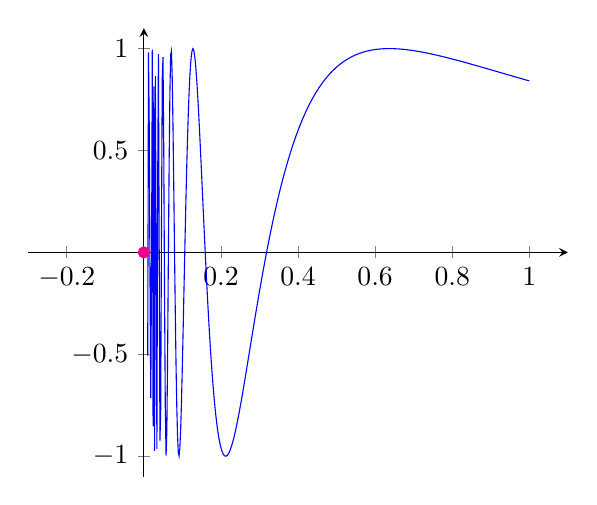
\begin{tikzpicture}
\begin{axis}[domain=0.01:1, xmin=-0.3, xmax=1.1, ymin=-1.1, ymax=1.1, samples=500, axis lines=middle]
\addplot[blue]{sin(deg(1/x))};
\draw[magenta, fill] (0,0) circle [radius=0.7mm];
\end{axis}
\end{tikzpicture}
\end{center}
Then, \(X\) is connected but not path-connected.

\begin{pf}
\underline{Connected}: Since \((0,1]\) is connected and the function
\(g(x)=(x,\sin 1/x)\) is continuous (as each component is continuous), \(A\) is
connected. Now consider any \(2\)-valued function \(f\) on \(X\). The
restriction \(f|_{A}\equiv C\) for some constant \(C\), due to the
connectedness of \(A\). Since \((0,0)\in\overline{A}\) and \(f\) is continuous,
\(f((0,0))=C\) also (by \Cref{prp:adher-accum-seq-equiv,prp:cts-seq-lim-crit}),
implying that \(f\) is constant.

\underline{Not path-connected}: Assume to the contrary that \(X\) is
path-connected. Then there exists a path \(\gamma:[0,1]\to X\) such that
\(\gamma(0)=(0,0)\) and \(\gamma(1)=(1/\pi,0)\). Note that the path can
``stay'' at \((0,0)\) for some time, but will eventually ``leave'' it since
\(\gamma(1)\ne (0,0)\). So, by removing the period of ``staying'' at \((0,0)\)
and scaling the remaining part accordingly, we can assume WLOG that
\(\inf\qty{t\in [0,1]: \gamma(t)\ne (0,0)}=0\), i.e., the path ``immediately''
leaves \((0,0)\) after the ``initial time point''.
\begin{center}
\begin{tikzpicture}
\draw[-Latex] (0,0) -- (10,0) node[right] {\(t\)};
\node[magenta] () at (2,0) {[};
\node[] () at (2,-0.5) {\(0\)};
\node[magenta] () at (8,0) {]};
\node[] () at (8,-0.5) {\(1\)};
\draw[blue, very thick] (2,0) -- (5,0);
\draw[blue, very thick] (5,0) .. controls (6,2) and (7,-2) .. (8,0);
\end{tikzpicture}
\begin{tikzpicture}
\draw[-Latex, orange, ultra thick] (5,3) -- (5,1);
\draw[-Latex] (0,0) -- (10,0) node[right] {\(t\)};
\node[magenta] () at (2,0) {[};
\node[] () at (2,-0.5) {\(0\)};
\node[magenta] () at (8,0) {]};
\node[] () at (8,-0.5) {\(1\)};
\draw[green!50!black, very thick] (2,0) .. controls (4,2) and (6,-2) .. (8,0);
\end{tikzpicture}
\end{center}

By the continuity of \(\gamma\), there exists \(\delta_0>0\) such
that for any \(t<\delta_0\), \(\|\gamma(t)-(0,0)\|<\frac{1}{2}\).

By the assumption about the infimum, there exists a sequence \(\{t_n\}\to 0\)
such that \(\gamma(t_n)\ne (0,0)\) for any \(n\in\N\). Then, choose a
\(0<t_{n_1}<\delta_0\) and choose \(N_1\in\N\) such that
\(N_1\pi<\frac{1}{t_{n_1}}<(N_1+1)\pi\). Next, choose
\(\displaystyle
0<t_{n_2}<\frac{1}{4N_1\pi}<\frac{1}{(N_1+1)\pi}<t_{n_1}<\delta_0\) such that
\(\gamma(t_{n_2})\ne (0,0)\).

Note that these choices of \(t_{n_1}\) and \(t_{n_2}\) are sufficiently far
apart that the path \(\gamma\) reaches at least one ``peak'' between
\(t_{n_1}\) and \(t_{n_2}\), i.e., there exists \(s\in(t_{n_1},t_{n_2})\) such
that \(\gamma(s)=(x,1)\) for some \(x\in (0,1]\).

Note that \(\gamma(t_{n_1}),\gamma(t_{n_2})\in \gamma([0,\delta_0])\). Since
\(\gamma([0,\delta_0])\) is connected, we conclude that every point \(p\)
``between'' \(\gamma(t_{n_1})\) and \(\gamma(t_{n_2})\), i.e., \(p\) with
\(p=\gamma(u)\) where \(u\in(t_{n_1},t_{n_2})\), belongs to
\(\gamma([0,\delta_0])\) as well, for otherwise, one can construct two nonempty
disjoint open subsets of \(\gamma([0,\delta_0])\) whose union is
\(\gamma([0,\delta_0])\), through splitting based on the ``missing point''.
\begin{center}
\begin{tikzpicture}
\draw[blue, fill] (0,0) circle [radius=0.5mm];
\draw[blue, fill] (4,0) circle [radius=0.5mm];
\draw[violet, very thick] (0,0) .. controls (1,2) .. (1.95,0.05);
\draw[green!50!black, very thick] (2.05,-0.05) .. controls (3,-2) .. (4,0);
\draw[red] (2,0) circle [radius=0.7mm];
\end{tikzpicture}
\end{center}

Particularly, it means that \((x,1)=\gamma(s)\in \gamma([0,\delta_0])\). But
\(\|\gamma(s)-(0,0)\|=\|(x,1)-(0,0)\|>1>1/2\), contradiction.
\end{pf}
\end{enumerate}
